%% Bemærk:
%%          Resten af rapporten følger en stil hvor indledninger skrives
%%          med \sffamlily-typen. Denne stil bør også følges her.
%%
{\sffamily
I vores program er, der fire forskellige tærskelværdier som påvirker
hvordan maleriet analyseres, når regionerne udtrækkes af maleriet.
Marginbredde, kantdetektion, floodfill og sløring. I denne sektion vil
vi finde værdier for de fire tærskelværdier, samt give en forklaring på hvorfor vi
har valgt lige de tal. Malerierne som er brugt i afprøvning er specielt
udvalgt for deres illustrative aspekt. 
}

\subsection{Størrelsen på margin}
Vi regner marginbredde ud fra en procentstats, kaldet $\Delta$, af
billedets $B$ og $H$. I defination \ref{margin_min} i afsnit \ref{margin_udregning} definerede vi den
minimale størrelse på margin til $2.1 \%$. Så $\Delta$ skal være større end $2.1 \%$. 

Den minimale forskel mellem to snit, som vi regner med at skulle sammenligne, er
det gyldne snit og $\frac{2}{3}$. I definition \ref{margin_max} sættes den
maksimale bredte af en margin til $2.43\%$. For at de to snits margin ikke
overlapper, skal $\Delta$ være mindre end $2.43\%$. 

Det vil sige at $\Delta \in [2.1, 2.43]$. Vi har valgt at
sætte $\Delta = 2.4$, da vi derved kan tage højde for uforudsete
usikkerheder.

\subsection{Afvigelsen af farver i kantdetektion}
Formålet med kantdetektion er at indkredse regioner, som vi finder
interessante. Kantdetektion finder dog også kanter inde i regionerne,
hvilket er en negativ sideeffekt. Vi skal nå et kompromis mellem 
perfekte kanter rundt om regionerne og undgå for mange kanter inden i regionerne.
. Dette gøres ved at ændre to tærskelværdier
i kantdetektionen. Vi har valgt at dele billederne som vi observerer op
i ni kategorier, se tabel \ref{thressholdsTabelKant}. Kategorierne er en
grov opdeling af billederne efter detaljer og farveintensitet, som
bruges til at give en bedre indblik i billedets opbygning.

\subsubsection{Sammenligninger}
Vi har undersøgt på ni malerier og har fundet de tærskelværdier, vi mener
passer bedst på malerierne. Vi vil illustrere, hvordan vi har fastsat
tærskelværdierne, på maleriet \ref{kDetalier}.

Maleriet er malet med mange farver og har mange detaljer. Vi ser først
på tærskelværdierne $(0,0),(100,100).....(600,600),(700,700)$. I
figurene \ref{allesammen1} og \ref{allesammen2} kan man se hvordan de
forskellige tærskelværdier påvirker hvad kantdetektoren finde af kanter i
billedet, læg mærke til at jo højere tærskelværdierne er, jo færre kanter
bliver der også fundet, og det blive sværere og sværere at genkende maleriet i kanterne. 

Vi finder det billede i \ref{allesammen1} og \ref{allesammen2}, med
højest tærskelværdi, som ikke har mistet for mange kanterne rundt om
regionerne endnu. Vi vurderer at billedet \ref{300-300} passer bedst på
den beskrivelse, da regionerne som vingerne, hoved og kroppen stadig er
omkranset af en kant. Så tærskelværdien $(300-300)$ er den værdi som får
vores kantdetektor til at virke bedst, indtil videre.

Ved gradvist at øge en af tærskelværdierne lidt op af gangen, kan vi finde en
bedre tærskelværdi for kantdetektoren. Vi opstiller igen en række
billeder med forskellige tærskelværdier og vurderer billederne ud fra
samme kriterier. Vi vurderer her at billedet \ref{300-750} passe bedst,
da vingerne, hoved og kroppen stadig har mange af deres kanter. Vi har
derfor valgt $(300-750)$ som tærskelværdi, da vi vurderer at netop denne
værdi er det bedste kompromis mellem kanter rundt om regioner og få
kanter indeni regionerne.

Det brugte maleri er ikke særlig repræsentativt for hele vores
billeddatabase. Så vi har også brugt metoden på otte andre billeder. Et
lille udsnit af de otte billeder kan ses i figur \ref{en}, \ref{to} og
\ref{tre}, hvor man skal lægge mærke til, hvorledes at de
kantdetekterede billeder nærmer sig et omrids af det originale billedes
regioner.

\clearpage
\begin{figure}[p]
    \centering
    \subfloat[Det original maleri. Navn: The Archangel Michae. År: Ca 1490 Af: Abadia, Juan de la]{
        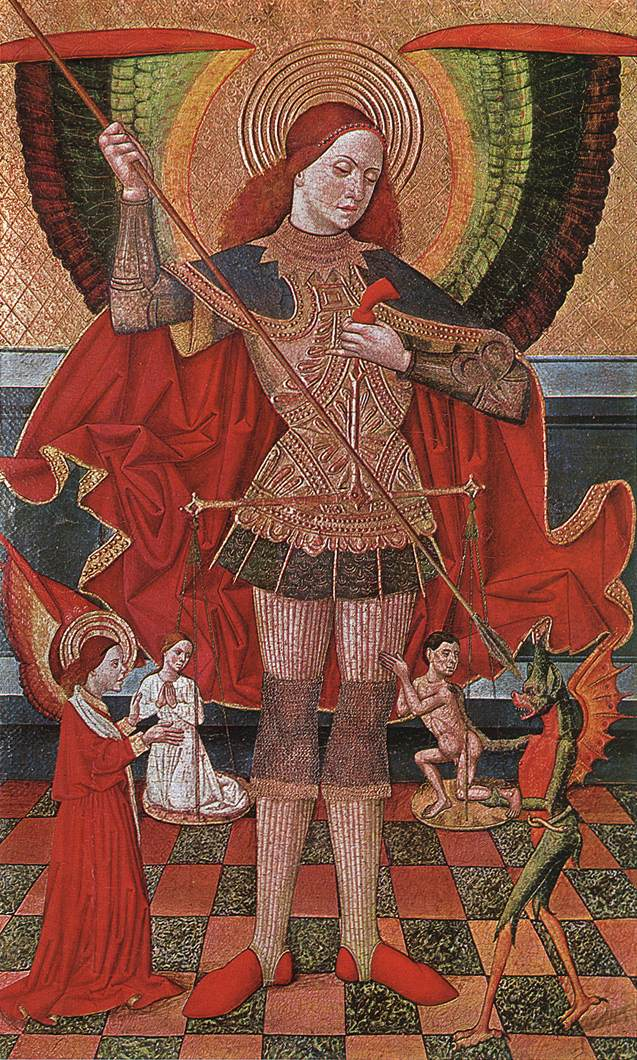
\includegraphics[angle=0,width=0.45\textwidth]{afsnit/afprovning/billeder/thressholds/krafitige_farver/krafite_detalier/kDetalier.jpg}
        \label{kDetalier}}
    \subfloat[(100,100)]{
        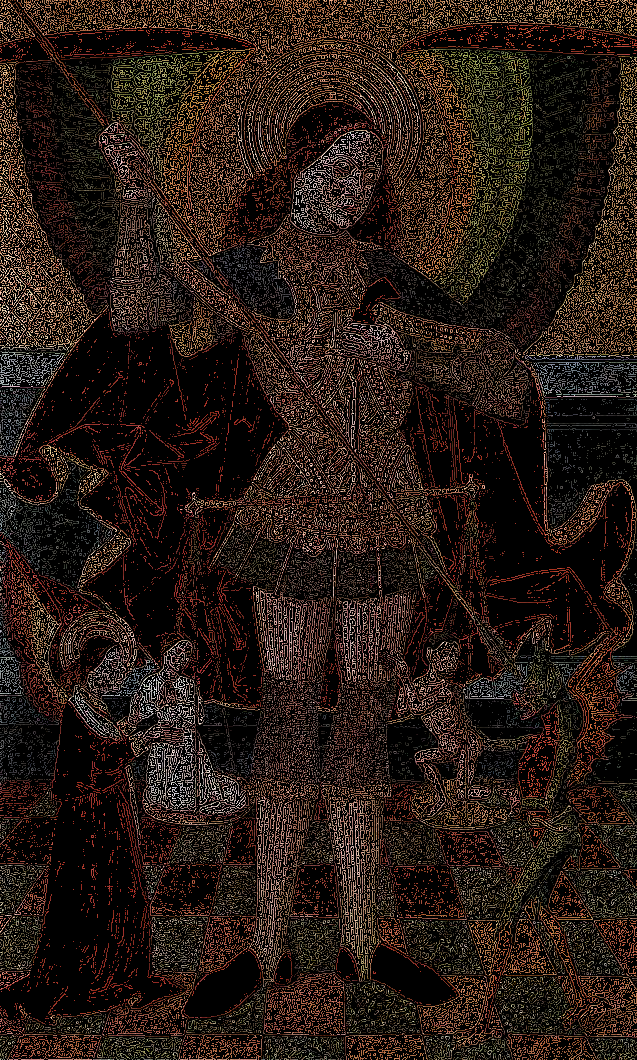
\includegraphics[angle=0,width=0.45\textwidth]{afsnit/afprovning/billeder/thressholds/krafitige_farver/krafite_detalier/1_iteration/100-100.png}
        \label{100-100}}\\
    \subfloat[(200,200)]{
        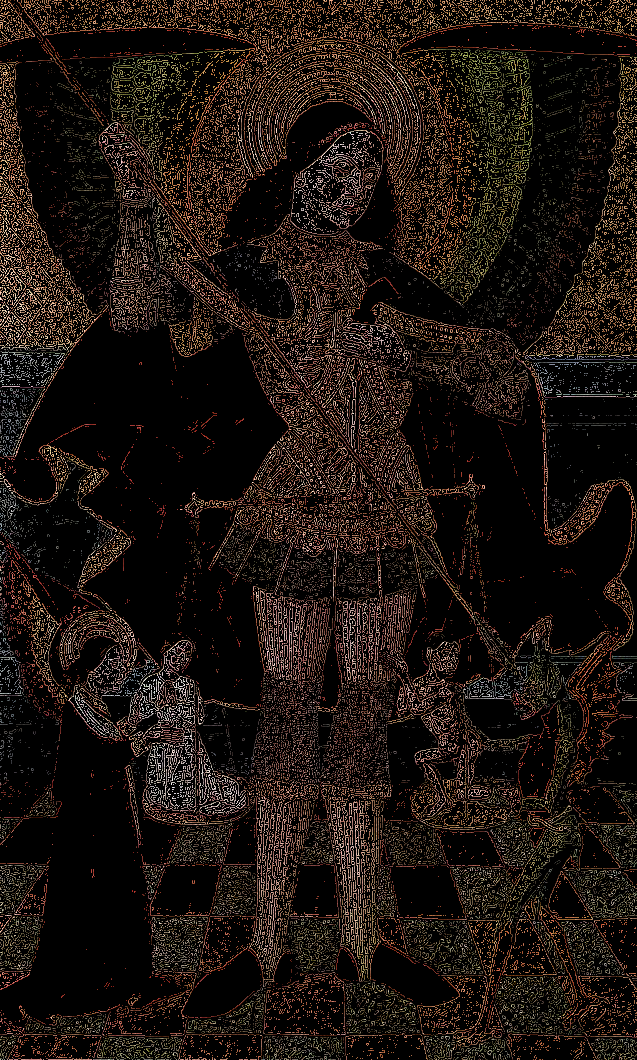
\includegraphics[angle=0,width=0.45\textwidth]{afsnit/afprovning/billeder/thressholds/krafitige_farver/krafite_detalier/1_iteration/200-200.png}
        \label{200-200}}
    \subfloat[(300,300)]{
        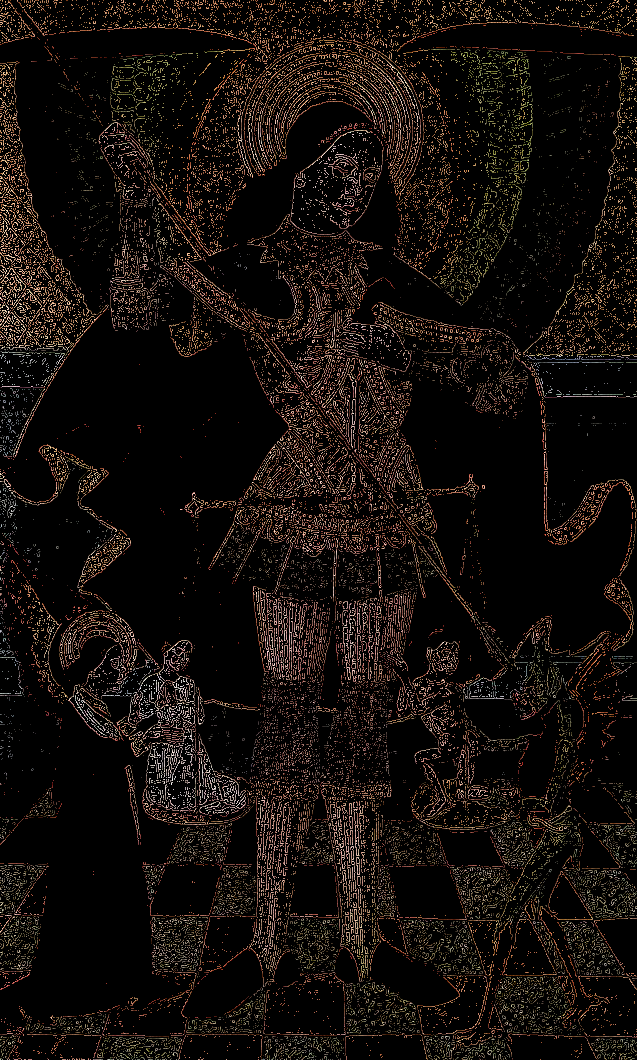
\includegraphics[angle=0,width=0.45\textwidth]{afsnit/afprovning/billeder/thressholds/krafitige_farver/krafite_detalier/1_iteration/300-300.png}
        \label{300-300}}\hspace{1em}
    \caption{Kantdetektion på maleriet \ref{kDetalier} som har mange
	detaljer og kraftige farver, med tærskelværdierne fra (100-100) til
	(300-300).}
	\label{allesammen1}
\end{figure}

\clearpage

\begin{figure}[!h]
	\centering
    \subfloat[(400,400)]{
        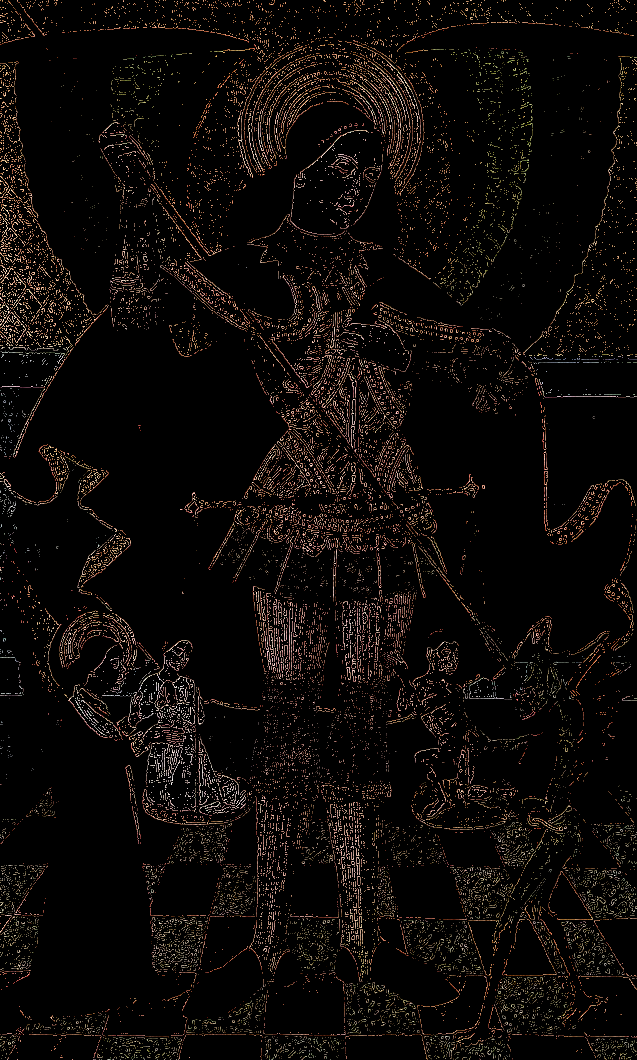
\includegraphics[angle=0,width=0.45\textwidth]{afsnit/afprovning/billeder/thressholds/krafitige_farver/krafite_detalier/1_iteration/400-400.png}
        \label{400-400}}    
	\subfloat[(500,500)]{
        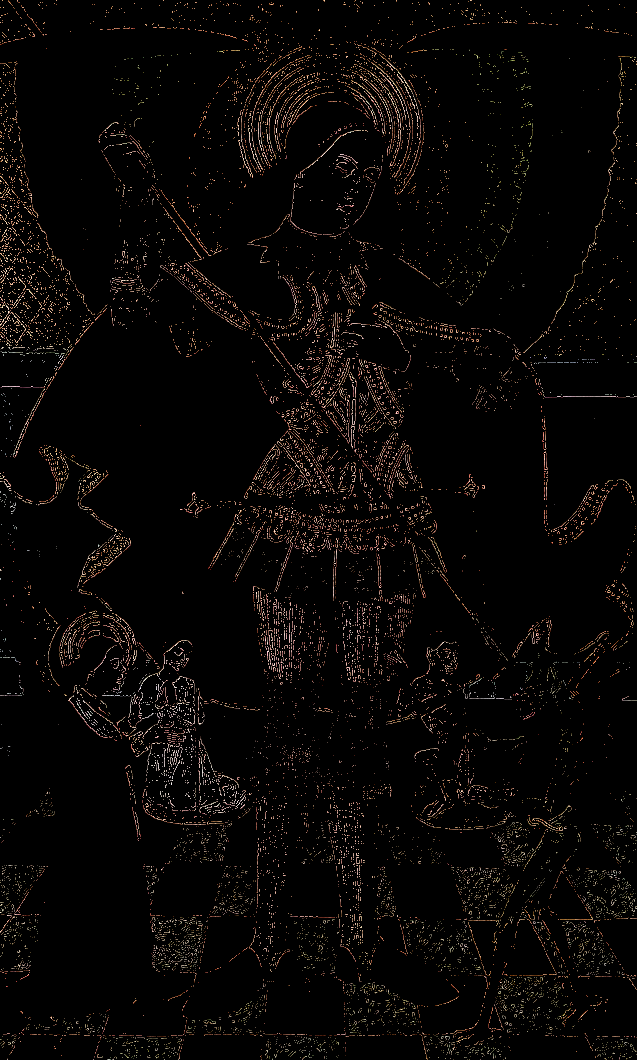
\includegraphics[angle=0,width=0.45\textwidth]{afsnit/afprovning/billeder/thressholds/krafitige_farver/krafite_detalier/1_iteration/500-500.png}
        \label{500-500}}\\
    \subfloat[(600,600)]{
        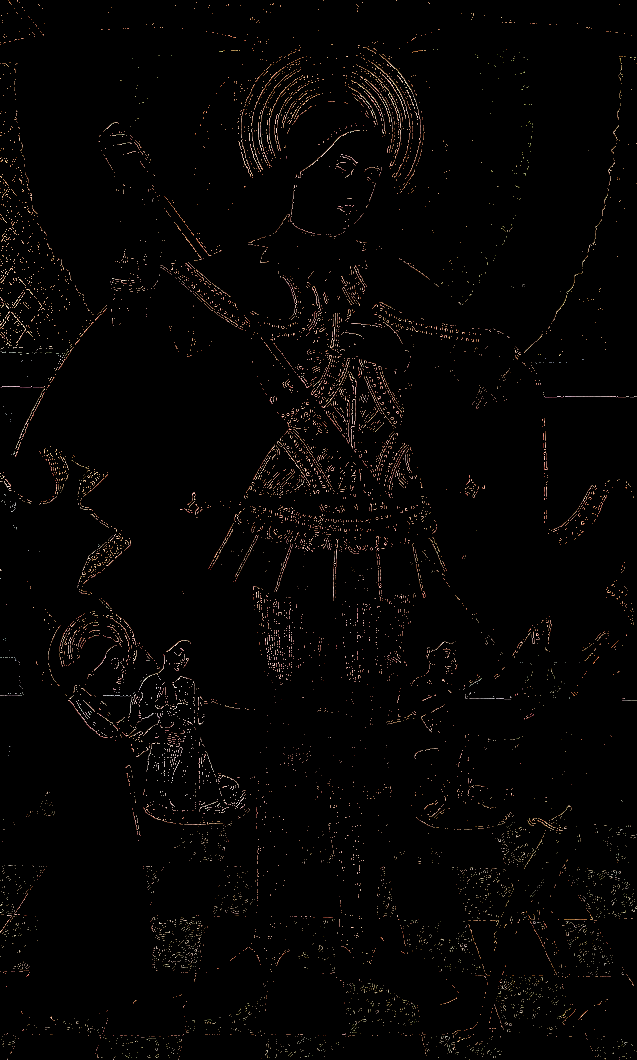
\includegraphics[angle=0,width=0.45\textwidth]{afsnit/afprovning/billeder/thressholds/krafitige_farver/krafite_detalier/1_iteration/600-600.png}
        \label{600-600}}
    \subfloat[(700,700)]{
        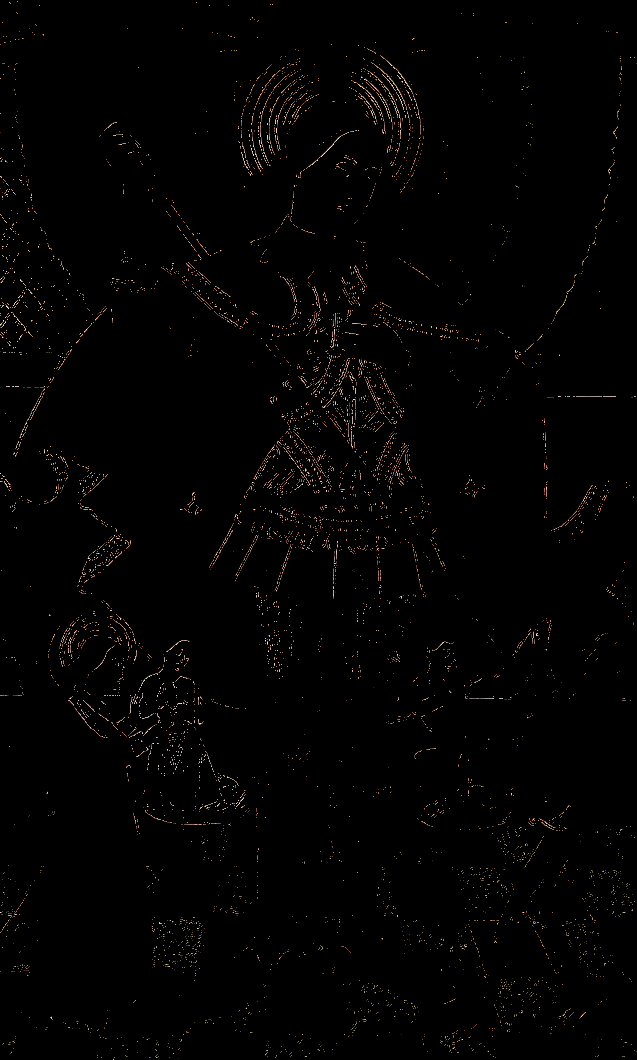
\includegraphics[angle=0,width=0.45\textwidth]{afsnit/afprovning/billeder/thressholds/krafitige_farver/krafite_detalier/1_iteration/700-700.png}
        \label{700-700}}
    \caption{Kantdetektion på maleriet \ref{kDetalier} som har mange
	detaljer og kraftige farver, med tærskelværdier fra (400-400) til
	(700-700).}
     \label{allesammen2}
\end{figure}

\begin{figure}[!h]
    \centering
    \subfloat[(300,700)]{
        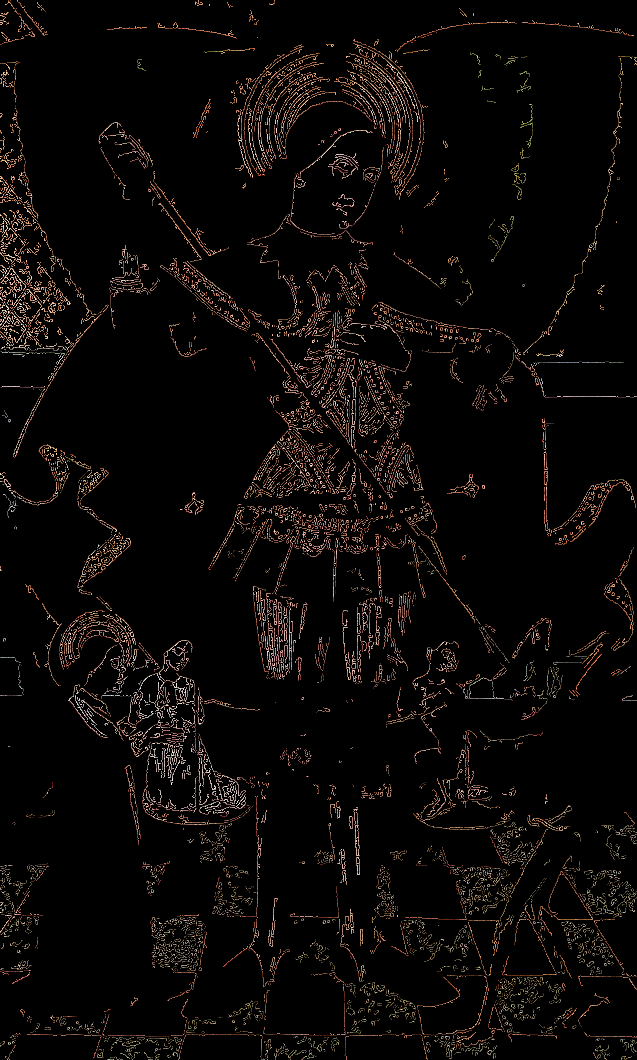
\includegraphics[angle=0,width=0.45\textwidth]{afsnit/afprovning/billeder/thressholds/krafitige_farver/krafite_detalier/2_iteration/300-700.png}
        \label{300-700}}\hspace{1em}
    \subfloat[(300,750)]{
        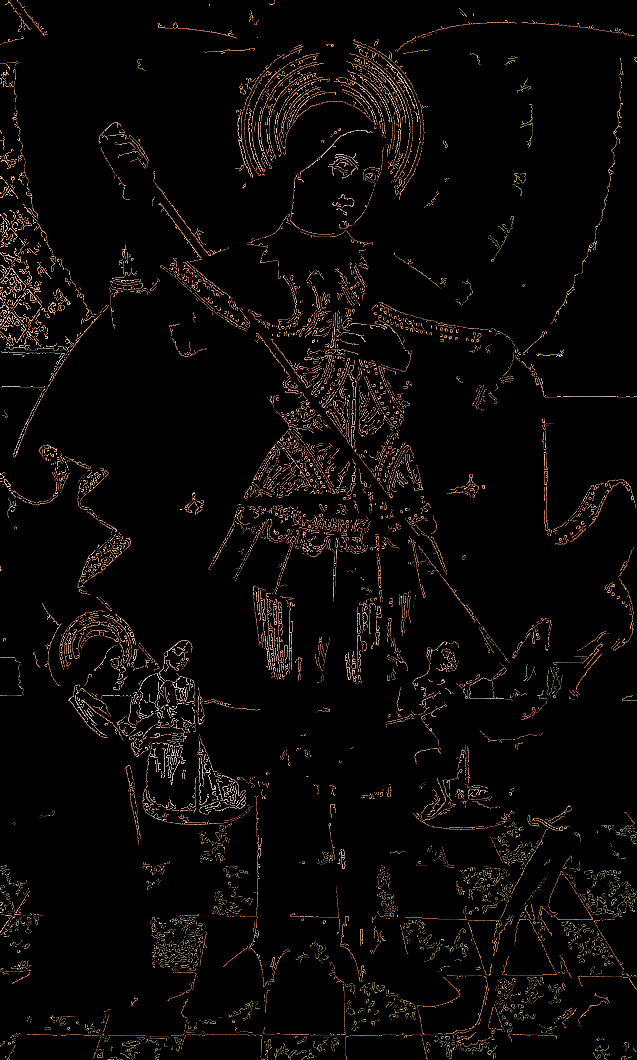
\includegraphics[angle=0,width=0.45\textwidth]{afsnit/afprovning/billeder/thressholds/krafitige_farver/krafite_detalier/2_iteration/300-750.png}
        \label{300-750}}\\
    \subfloat[(300,800)]{
        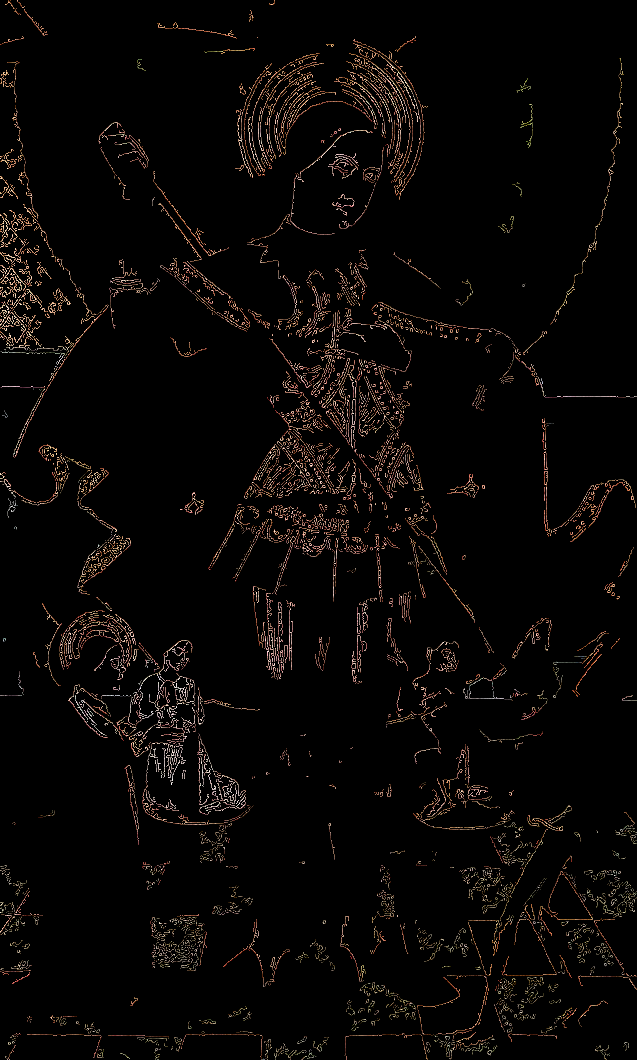
\includegraphics[angle=0,width=0.45\textwidth]{afsnit/afprovning/billeder/thressholds/krafitige_farver/krafite_detalier/2_iteration/300-800.png}
        \label{300-800}}\hspace{1em}
    \subfloat[(300,850)]{
        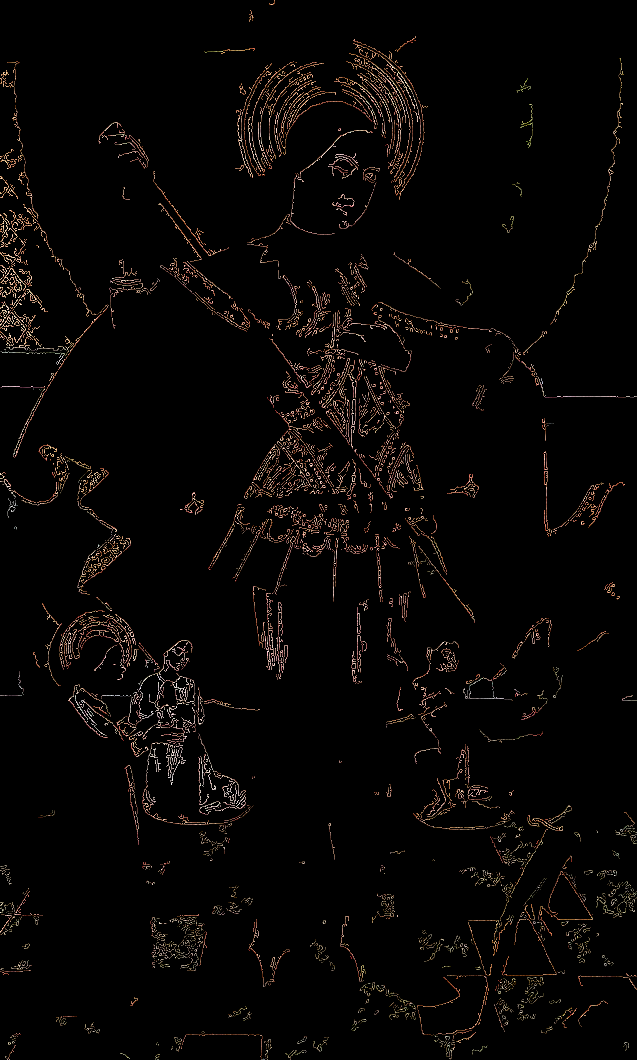
\includegraphics[angle=0,width=0.45\textwidth]{afsnit/afprovning/billeder/thressholds/krafitige_farver/krafite_detalier/2_iteration/300-850.png}
        \label{300-850}}
        \caption[]{Kantdetektion hvor de fire billeder som er
		interessante er taget med.}
     \label{allesammen3}
\end{figure}
 
\begin{figure}[!h]
    \centering
    \subfloat[Det original maleri. Navn: The Lamentation over St Francis. År: 1440. Af: Angelico, Fra. ]{
        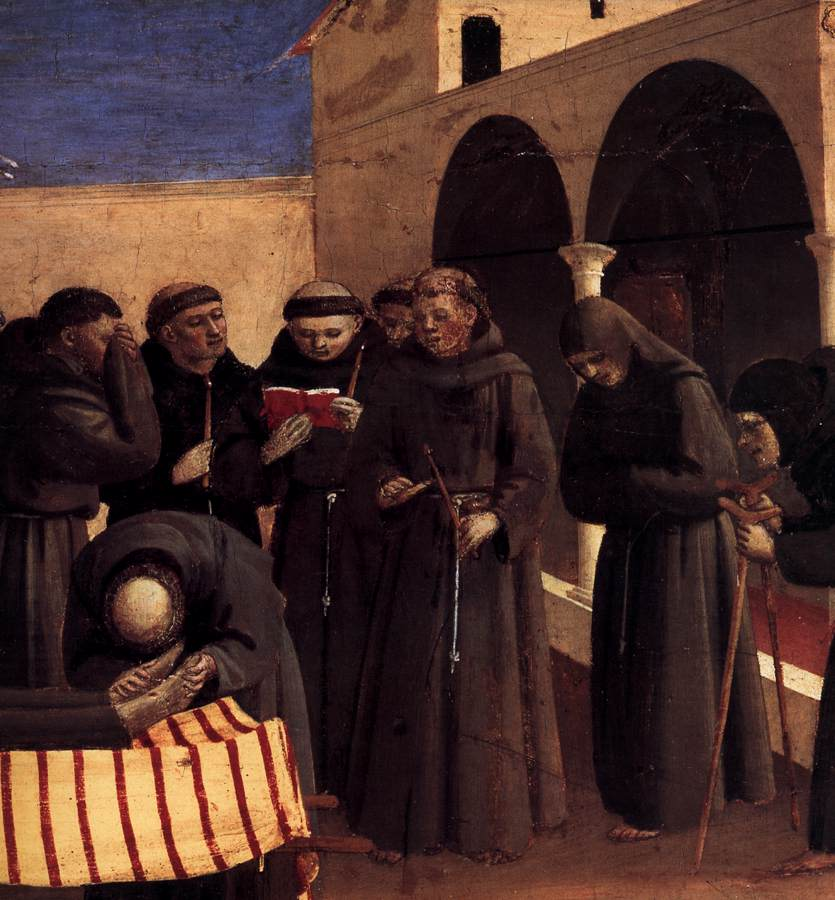
\includegraphics[angle=0,width=0.45\textwidth]{afsnit/afprovning/billeder/thressholds/svage_farver/svage_detalier/sDetalier.jpg}
        \label{Orginal1}}
    \subfloat[(100,250)]{
        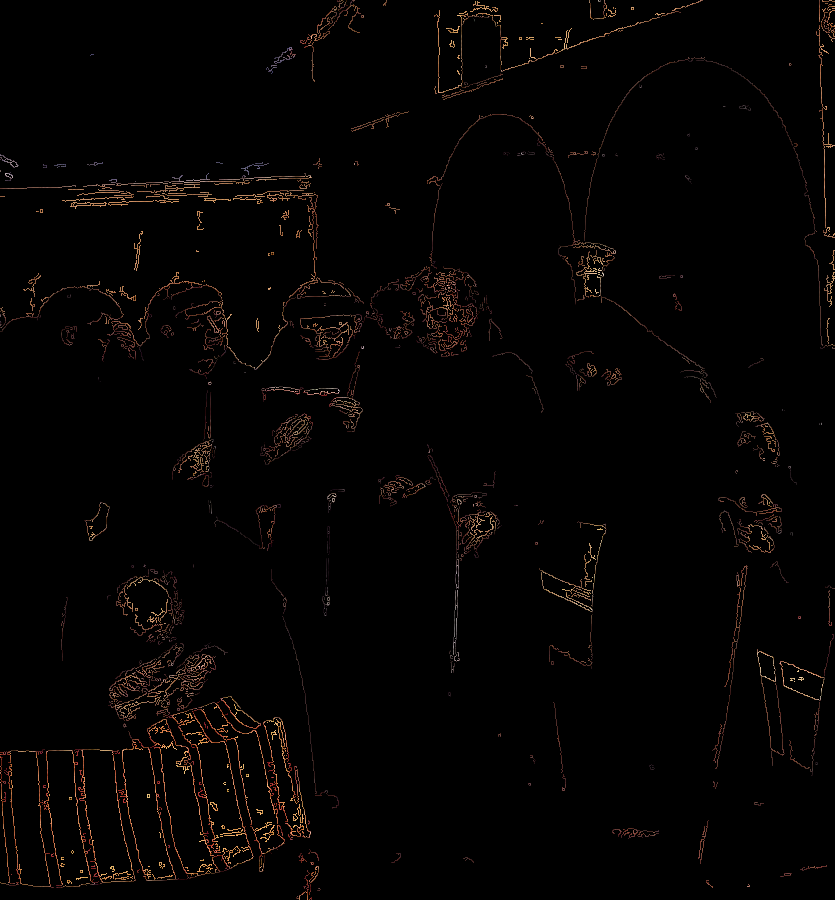
\includegraphics[angle=0,width=0.45\textwidth]{afsnit/afprovning/billeder/thressholds/svage_farver/svage_detalier/2_iteration/100-250.png}
        \label{100-250}}\hspace{1em}
        \caption[]{Kantdetektion på et billedet med svage farver og få detaljer, hvor tærskelværdien (100,250) er den bedste}
     \label{en}
\end{figure}

\begin{figure}[!h]
    \centering
    \subfloat[Det original maleri. Navn: The Ninth Wave. År: 1850. Af: Aivazovsky, Ivan Konstantinovich.]{
        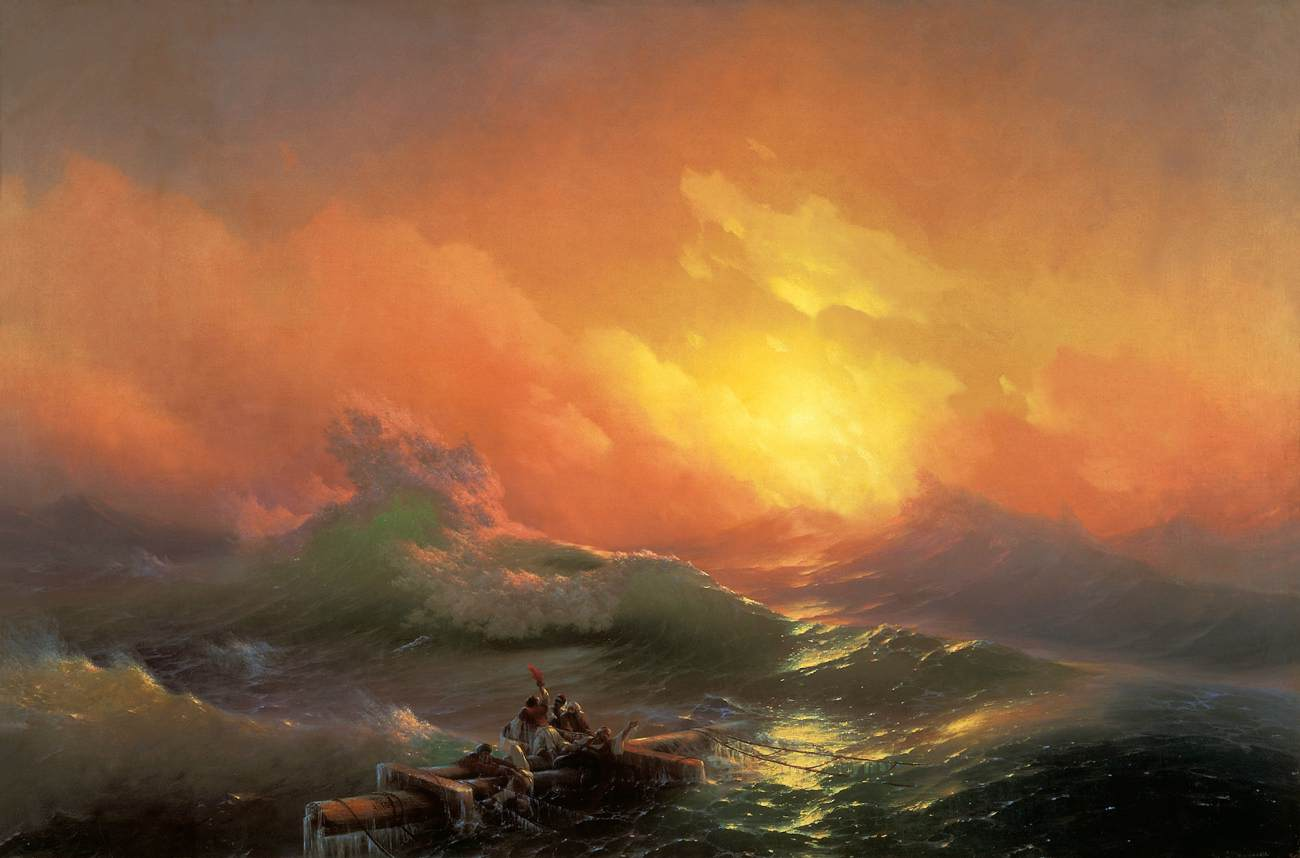
\includegraphics[angle=0,width=0.85\textwidth]{afsnit/afprovning/billeder/thressholds/medium_farver/svage_detalier/sDetalier1.jpg}
        \label{Orginal2}}\\
    \subfloat[(100,240)]{
        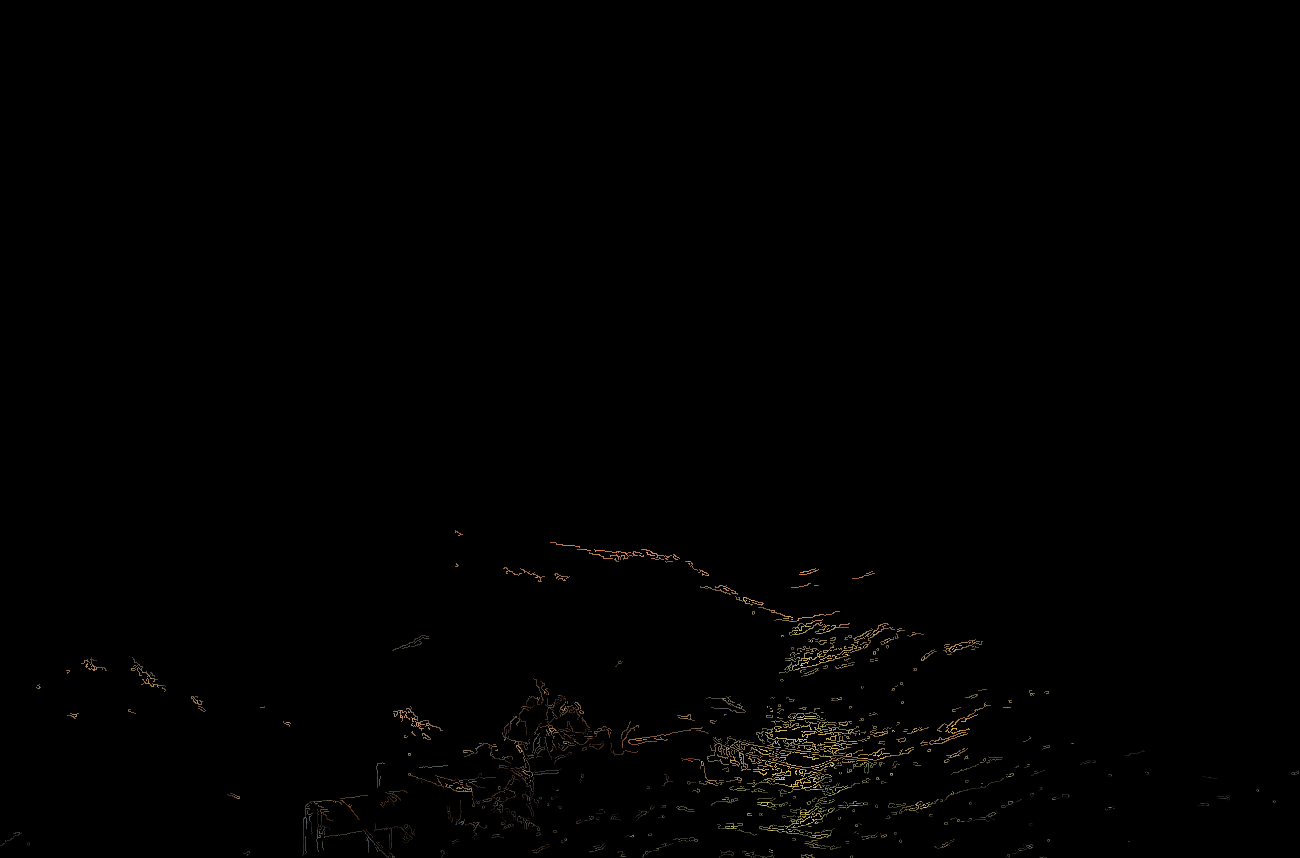
\includegraphics[angle=0,width=0.85\textwidth]{afsnit/afprovning/billeder/thressholds/medium_farver/svage_detalier/2_iteration/100-240.png}
        \label{100-240}}
        \caption[]{Kantdetektion på et billede med medium farver og få
		detaljer, hvor tærskelværdien (100,240) er den bedste.}
     \label{to}
\end{figure}

\begin{figure}[!h]
    \centering
    \subfloat[Det original maleri. Name: The last supper. År: 1498. Af:
	Leonardo da Vinci.]{
        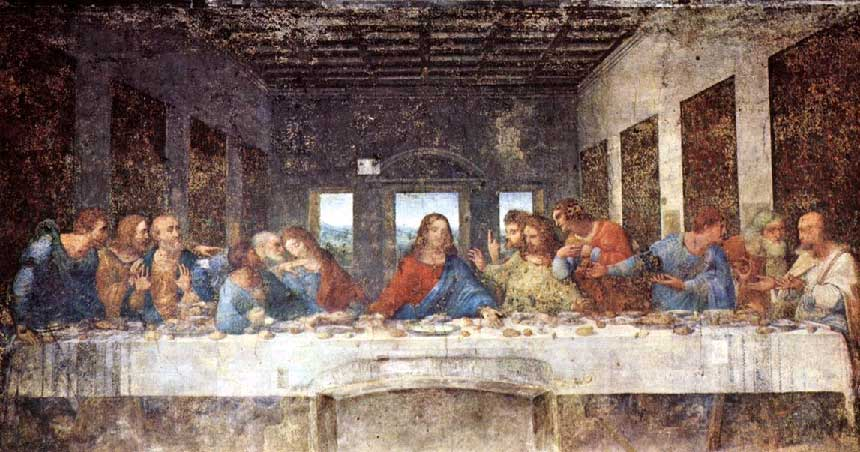
\includegraphics[angle=0,width=0.85\textwidth]{afsnit/afprovning/billeder/thressholds/medium_farver/medium_detalier/mDetalier1.jpg}
        \label{Orginal3}}\\
    \subfloat[(200,460)]{
        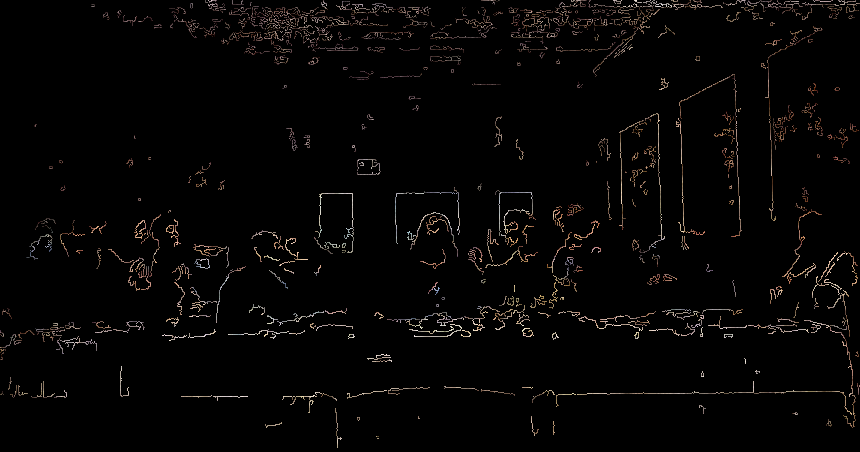
\includegraphics[angle=0,width=0.85\textwidth]{afsnit/afprovning/billeder/thressholds/medium_farver/medium_detalier/2_iteration/200-460.png}
        \label{200-460}}

        \caption[]{Kantdetektion på et billedet med medium farver og
		medium detaljer, hvor tærskelværdien [200,460] er den bedste.}
     \label{tre}
\end{figure}

\begin{table}[!h]
    \centering
    \begin{tabular}{| l | l | l | l |} \hline
        & Svage farver 	& Medium farver & Kraftige farver \\ \hline
        Få detaljer 		& (100,250)		& (100,240)		& (200,320)\\ \hline
        Medium detaljer 	& (100,280)		& (200,460)		& (200,380)\\ \hline
        Mange detaljer		& (200,400)		& (200,380)		& (300,750)\\ \hline
    \end{tabular}
    \caption{Tabel over kantdetektionstærskelværdier for ni malerier}
    \label{thressholdsTabelKant}
\end{table}

Det ses i tabel \ref{thressholdsTabelKant} går tærskelværdierne
fra $(100,240)$ til $(300,750)$, så vi tager en gennemsnit af værdierne
og få at de to tærskelværdier skal være $(177,384)$. 

Vi har dog i vores forsøg regnet med værdierne $(78,194)$, da vores
indledende afprøvninger afviger en smule fra den denne afprøvning.

\subsection{Afvigelsen af farver i floodfill}
Floodfill har to tærskelværdier $lo$ og $up$, som betegner hvor mange
pixelværdier en nabopixels farver må afvige. En
fyldestgørelses beskrivelse af floodfill findes i afsnit
\ref{section_opdeling}. 

Vi har tænkt os at finde en fælles tærskelværdi til brug i vores
program. Vi observere hvordan floodfill virker med forskellige
tærskelværdier og finder dem, som passer bedst til maleriet. Resultatet
for observationen kan ses i tabel \ref{thressholdsTabelFF}, hvor de
sammen ni kategorier er brugt og afprøvet på de samme ni malerier. Et af
de malerier hvor den optimale tærskelværdi er fundet kan ses i figur
\ref{Floodfillbilledet}, læg mærke til hvordan træet, samt
snebaggrunden, er fyldt næsten helt ud, uden at nogle af menneskerne er farvet over.

\begin{figure}[!h]
    \centering
    \subfloat[Det originale maleri. Navn: Winter Landscape. År: Ukent. Af: Avercamp, Hendrick.]{
        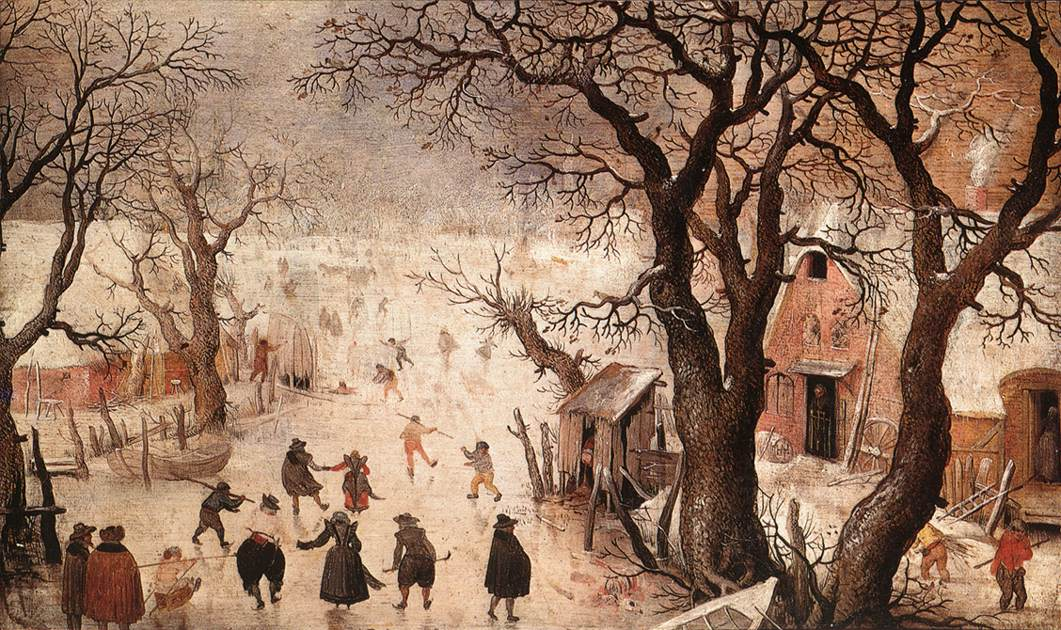
\includegraphics[angle=0,width=0.9\textwidth]{afsnit/afprovning/billeder/thressholds/svage_farver/kraftige_detalier/kDetalier.jpg}
        \label{Orginal4}}\\
    \subfloat[8,8]{
        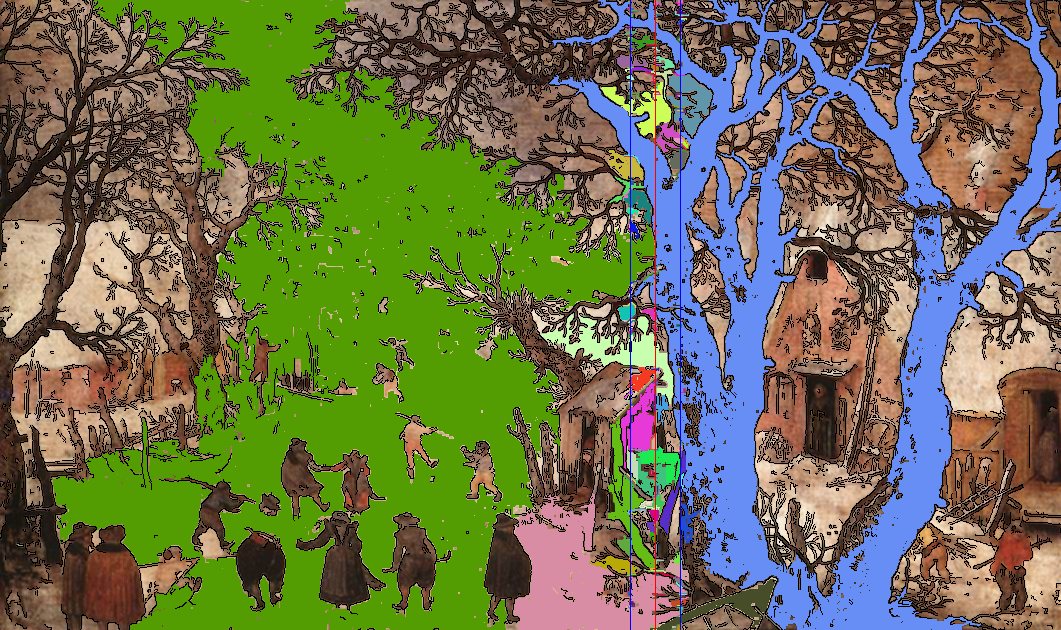
\includegraphics[angle=0,width=0.9\textwidth]{afsnit/afprovning/billeder/thressholds/svage_farver/kraftige_detalier/floodfill/8-8.png}
        \label{8-8}}
    \caption[]{Tærskelværdierne på et billede med svage farver og
	kraftige detaljer hvor tærskelværdien (8,8) passer bedst.}
    \label{Floodfillbilledet}
\end{figure}

\begin{table}[!h]
    \centering
    \begin{tabular}{| l | l | l | l |} \hline
        & Svage farver 		& Medium farver & Kraftige farver \\ \hline
        Få detalier 		& \textbf{(2,2)}	& (3,3)			& (4,4)\\ \hline
        Medium detalier 	& \textbf{(2,2)}	& \textbf{(5,5)}& \textbf{(2,2)}\\ \hline
        Mange detalier		& (8,8)				& (4,4)			& (7,7)\\ \hline
    \end{tabular}
    \caption{Tabel over floodfill tærskelværdier på ni malerier, tal med
    fed er for malerier hvor vi ikke har kunne finde en værdi som passe
    godt nok til at kunne sige at passe.}
    \label{thressholdsTabelFF}
\end{table}

Værdierne i tabel fluktuere også en del, så vi tager
gennemsnittet af værdierne, som ikke er markeret med fed og får en tærskelværdierne på (5,5).
